\chapter{Experimenten en Resultaten}
\label{hoofdstuk:ER}
In dit hoofdstuk worden de belangrijkste experimenten besproken die uitgevoerd in het verloop van deze masterproef. Deze hebben zowel betrekking op de besproken melodische transformaties, de algoritmes om deze transformaties te combineren en ook het RPK-model dat gebruikt werd om deze transformaties te evalueren.

\section{Transformaties combineren: 1 transformatie, meerdere iteraties}
\label{experiment:1}
\subsection{Beschrijving experiment}
Dit experiment heeft betrekking tot het algoritme dat besproken werd in onderdeel \ref{ETT:algo1}. Dit experiment gaat nagaan wat de invloed is van het aantal iteraties van het aantal iteraties van dit algoritme op de consonantiescore van het totale muziekstuk. Er wordt in dit algoritme slechts gebruik gemaakt van een transformatie. Deze gebruikte transformatie wordt weergegeven in tabel \ref{tabel:exp1}.

\begin{table}
  \centering
  \begin{tabular}{c | c c c c c c c c }
    Diff (mod 8) & 0 & 1 & 2 & 3 & 4 & 5 & 6 & 7 \\
    \hline
    \hline
    Verhoging & 5 & -4 & 1 & -3 & 1 & 1 & 2 & 3 \\
  \end{tabular}
  \caption{Transformatie gebruikt in het experiment van onderdeel \ref{experiment:1}.}
  \label{tabel:exp1}
\end{table}

Deze test wordt uitgevoerd op 100 muziekstukken uit het Essencorpus. De gemiddelde consonantiescore van de originele stukken wordt berekend alsook de gemiddelde consonantiescore van het muziekstuk dat optimaal is volgens het RPK-model in de toonaard van de 100 stukken. Nu kan er gekeken worden naar hoe snel de consonantiescore zich gaat verplaatsten van die van het originele naar die van de theoretisch best mogelijke volgens het model afhankelijk van het aantal iteraties dat het algoritme wordt uitgevoerd.

\subsection{Resultaten}

\begin{figure}[!ht]
  \centering
  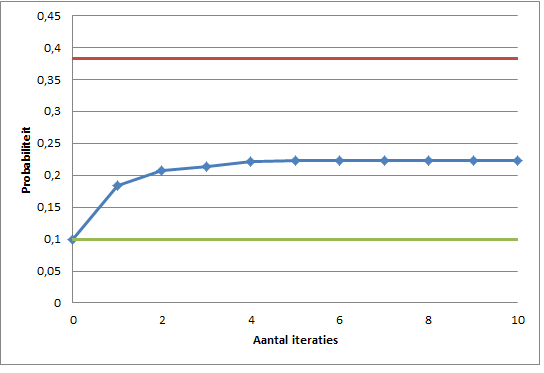
\includegraphics[width=0.75\textwidth]{5_Experimenten_Resultaten/exp1_res}
  \caption{Resultaten van het experiment uitgevoerd in deel \ref{experiment:1}. Groene lijn staat voor probabiliteit originele melodie, rode lijn voor de probabiliteit van het theoritisch beste lijn in de toonaarden waarop getest werd en de blauwe lijn geeft de probabiliteit weer na uitvoer van het algoritme na een verschillend aantal iteraties.}
  \label{figuur:exp1}
\end{figure}

\section{Transformaties combineren: meerdere transformaties, 1 iteratie}
\label{experiment:2}
\subsection{Beschrijving experiment}
Dit experiment heeft betrekking tot het algoritme dat besproken werd in onderdeel \ref{ETT:algo1}. Dit experiment gaat nagaan wat de invloed is van het aantal verschillende toegelaten transformaties op de consonantiescore van het totale muziekstuk. Zo zijn de vijf transformaties die gebruikt zullen worden weergegeven in tabel \ref{tabel:exp2}. Er wordt nu telkens slechts een iteratie van het algoritme uitgevoerd.

\begin{table}
  \centering
  \begin{tabular}{c | c c c c c c c c }
    Diff (mod 8) & 0 & 1 & 2 & 3 & 4 & 5 & 6 & 7 \\
    \hline
    \hline
    Verhoging transformatie 1 & 5 & -4 & 1 & -3 & 1 & 1 & 2 & 3 \\
    \hline
    Verhoging transformatie 2 & 1 & 3 & 4 & -5 & -1 & 6 & 5 & -1 \\
    \hline
    Verhoging transformatie 3 & 1 & 4 & 5 & -3 & 2 & -1 & 1 & 0 \\
    \hline
    Verhoging transformatie 2 & 4 & 6 & -2 & 4 & 2 & 6 & -4 & 2 \\
    \hline
    Verhoging transformatie -2 & -3 & -2 & 3 & -1 & 4 & -3 & 2 & -4 \\
  \end{tabular}
  \caption{Transformaties gebruikt in het experiment van onderdeel \ref{experiment:2}.}
  \label{tabel:exp2}
\end{table}

\subsection{Resultaten}

\section{Transformaties combineren: minimum transformatie lengte}
\label{experiment:3}
\subsection{Beschrijving experiment}

\subsection{Resultaten}

\section{Transformaties combineren: Gelijkheid algoritmen voor transformatie lengte 1}
\label{experiment:4}
\subsection{Beschrijving experiment}

\subsection{Resultaten}

\section{Vergelijking transformatie scores}
\label{experiment:5}
\subsection{Beschrijving experiment}

\subsection{Resultaten}

\section{Invloed rij van Fibonacci op transformaties}
\label{experiment:6}
\subsection{Beschrijving experiment}

\subsection{Resultaten}

\section{Test Performantie algoritmes}
\label{experiment:7}
\subsection{Beschrijving experiment}

\subsection{Resultaten}

%%% Local Variables: 
%%% mode: latex
%%% TeX-master: "masterproef"
%%% End: 
